\documentclass[10pt,a4paper,titlepage]{report}
\usepackage[utf8]{inputenc}
\usepackage{amsmath}
\usepackage{amsfonts}
\usepackage{amssymb}
\usepackage{graphicx}
\usepackage{color}

\begin{document}
\begin{titlepage}
\author{Rwithik Manoj}
\title{Setting up a Version Control System with Git}
\date{\today}
\maketitle
\end{titlepage}
\begin{center}
\Large{The Local Repository}
\end{center}
\vspace{.5cm}
\par The first step in using a version control system is making the actual repository. Here, I've made a directory named `foss-lab' and converted it into a git repo by using {\color{red} git init} inside the directory. This creates a .git directory inside the repo, which store the details about the git version control system. This directory is our local repository. I've also made a README.md file. \newline
\newline
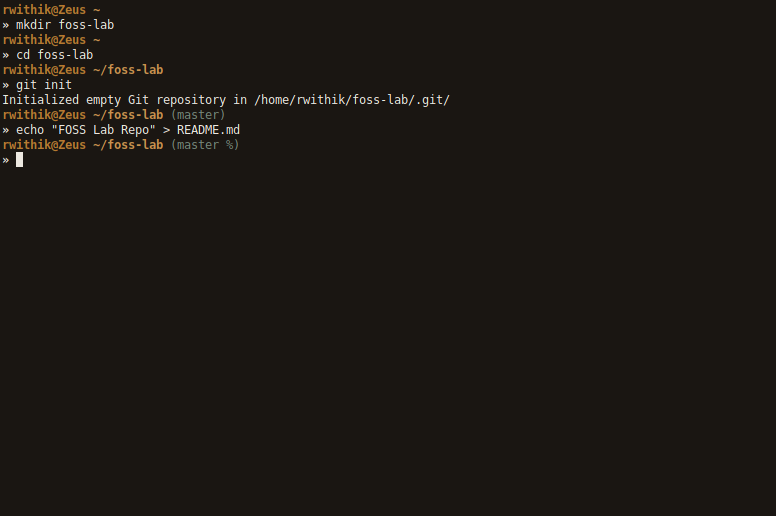
\includegraphics[scale=.45]{../Images/VCS/1.png}
\pagebreak
\begin{center}
\Large{The Remote Repository}
\end{center}
\vspace{.5cm}
\par The local repository exists only on my system. We need to connect it to a remote repository, for any sort of collaboration to be possible. So, I made an online repo at github.com. \newline\newline
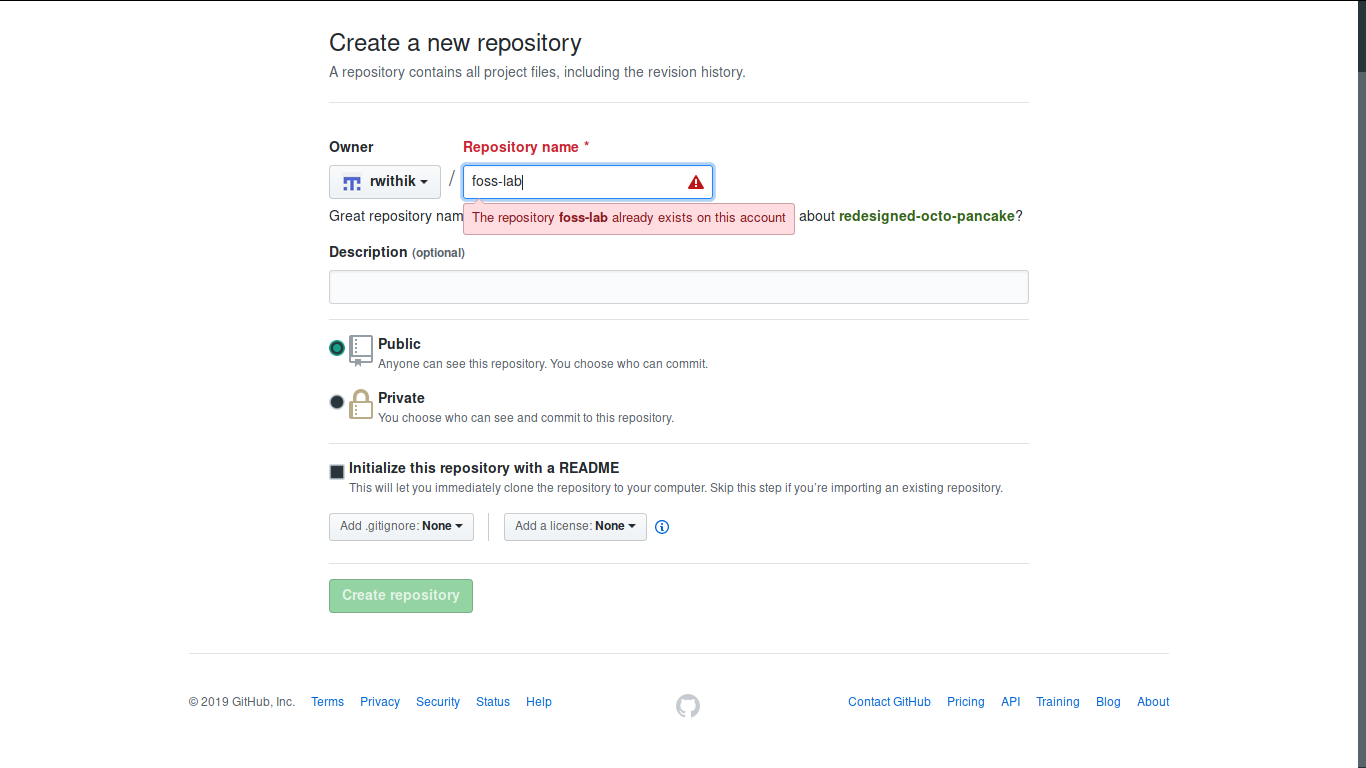
\includegraphics[scale=.25]{../Images/VCS/github.png}\newline
\par Now we need to connect the local repo to the  online repo. This is done using the {\color{red} git remote} command. \newline
Syntax: git remote add origin [URL] \newline\newline
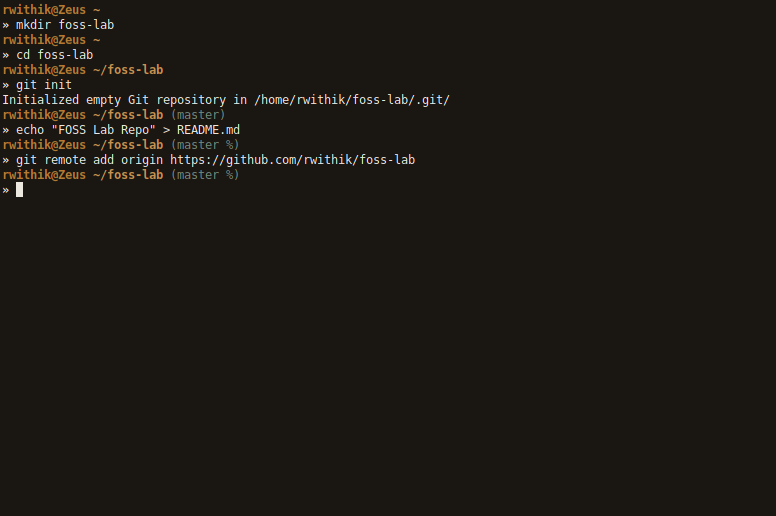
\includegraphics[scale=.45]{../Images/VCS/2.png}
\pagebreak
\begin{center}
\Large{Making Changes}
\end{center}
\vspace{.5cm}
\par Any new files or any changes in existing files should be added to the local and remote repositories. This is done with the {\color{red} git add} command. This add the modified and new files to the staging area. Then the files are committed with a commit message using {\color{red} git commit}. This records the changes in the local repo. \newline
Syntax: git add [FILE(S)]\newline
git commit -m "MESSAGE"
\newline\newline
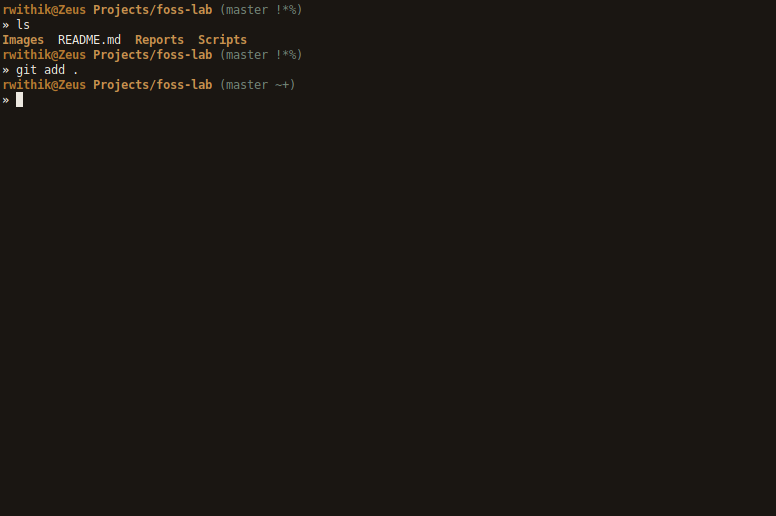
\includegraphics[scale=.45]{../Images/VCS/3.png}\newline\newline
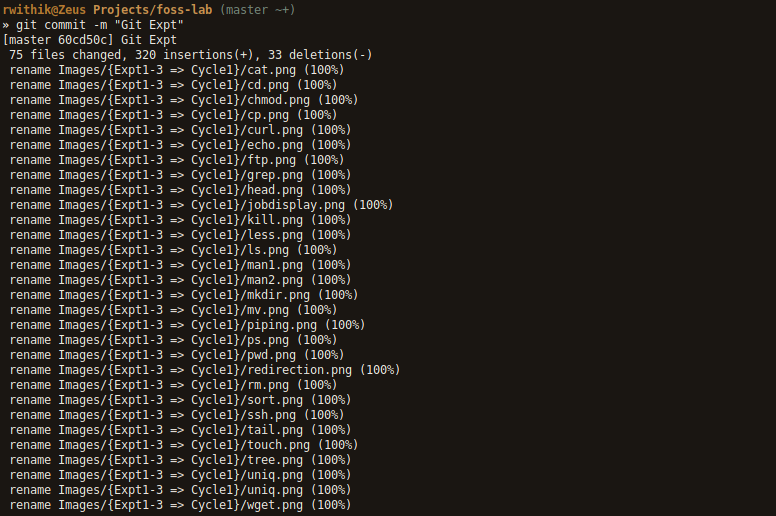
\includegraphics[scale=.45]{../Images/VCS/4.png}
\begin{center}
\Large{Pushing Changes to the Remote Repository}
\end{center}
\vspace{.5cm}
\par The changes we committed are currently recorded in the local repository. To push these changes to the remote repo, use {\color{red} git push}. In the example given below, origin is the name of the remote, and master is the name of the branch. \newline\newline
Syntax: git push [REMOTE NAME] [BRANCH NAME]
\newline\newline
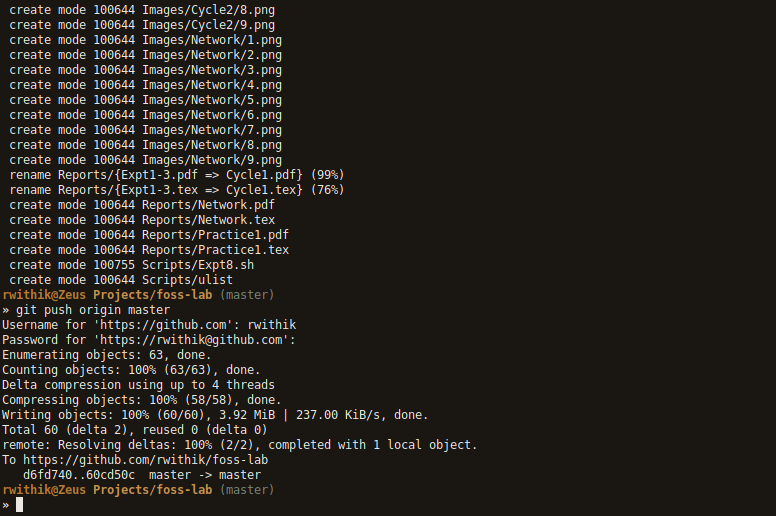
\includegraphics[scale=.45]{../Images/VCS/5.png}
\pagebreak
\begin{center}
\Large{Comparing Previous Versions}
\end{center}
\vspace{.5cm}
\par Use the {\color{red} git log} command to see all the previous changes with their commit messages. \newline\newline
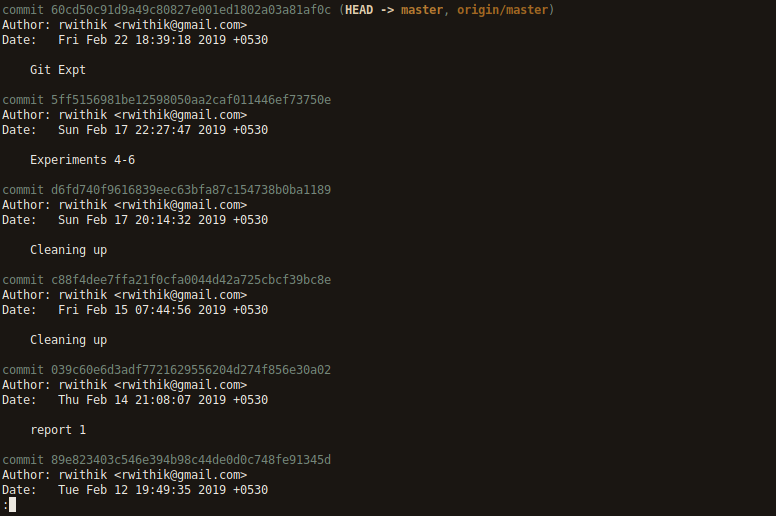
\includegraphics[scale=0.45]{../Images/VCS/6.png}\newline\newline
Use {\color{red} git checkout} to revert to a previous state of the repo. \newline
Syntax: git checkout [BRANCH]
\newline\newline
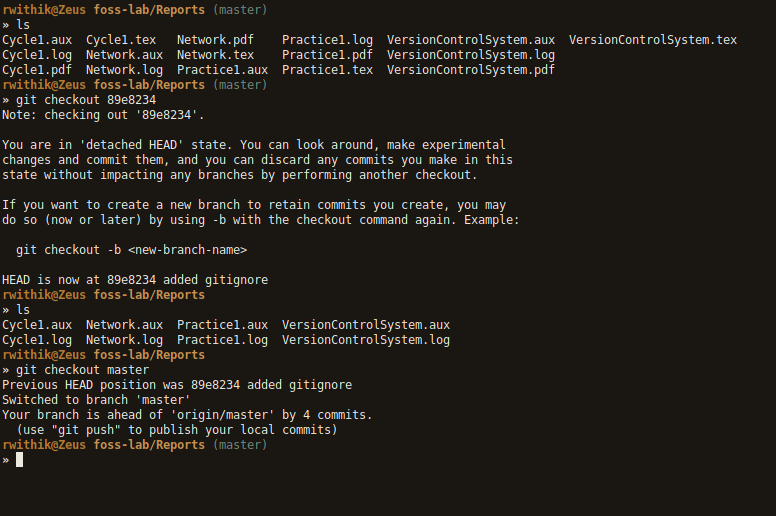
\includegraphics[scale=.45]{../Images/VCS/10.png}
\pagebreak
\begin{center}
\Large{Merge Conflicts}
\end{center}
\vspace{.5cm}
\par The {\color{red} git pull} command is used to update the local repo when it is behind the remote repo. Automatic merges of changed files occur normally, but in cases where the same lines are changed in both the repos, a merge conflict occurs. It can be resolved by editing the conflicted files and choosing which change to keep. \newline\newline
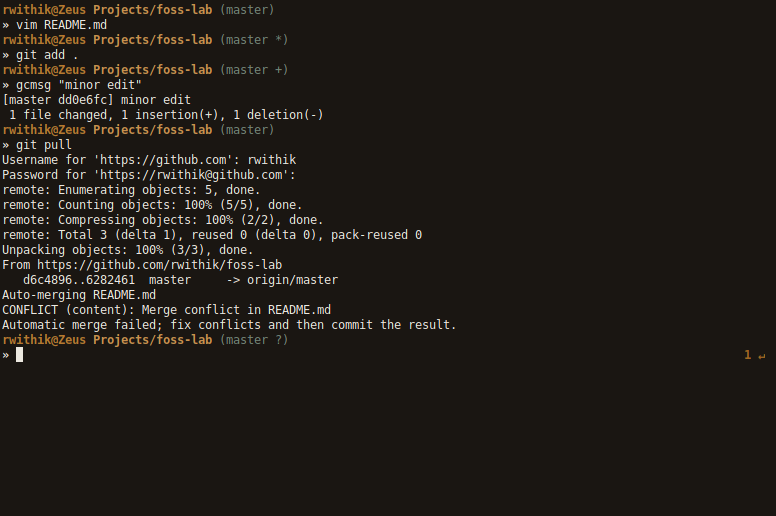
\includegraphics[scale=.45]{../Images/VCS/7.png}\newline\newline
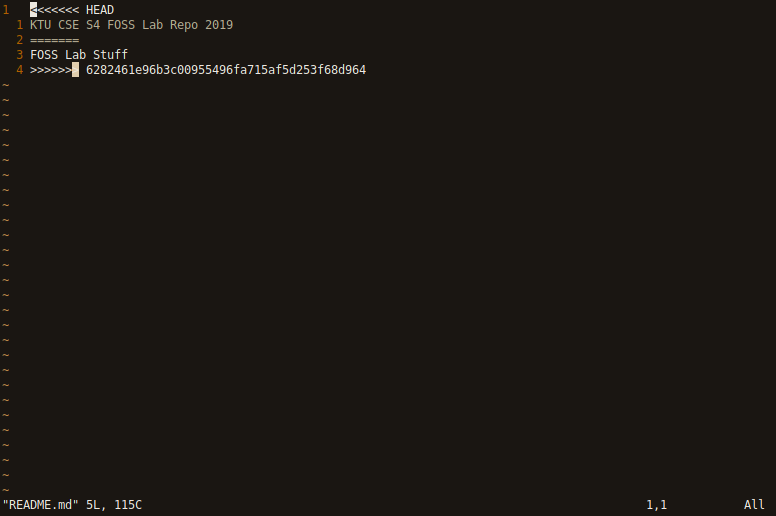
\includegraphics[scale=.45]{../Images/VCS/8.png}\newline\newline
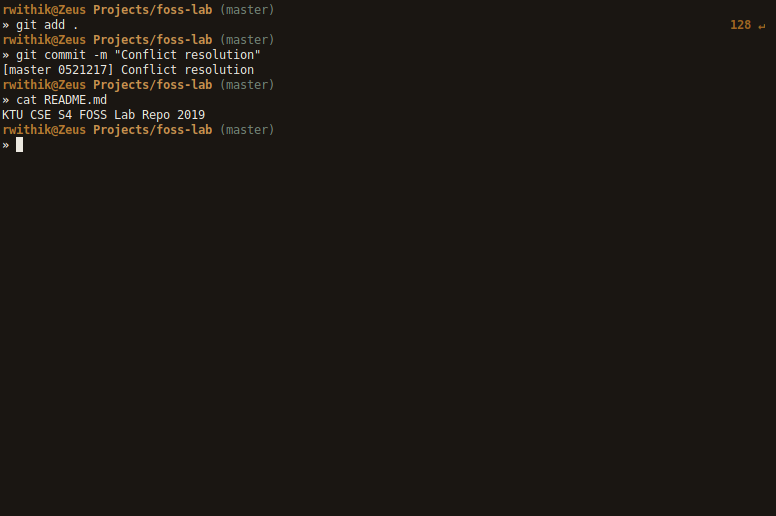
\includegraphics[scale=.45]{../Images/VCS/9.png}
\end{document}